% DO NOT COMPILE THIS FILE DIRECTLY!
% This is included by the other .tex files.

\begin{frame}[t,plain]
\titlepage
\end{frame}

\begin{frame}
	\frametitle{Agenda}
	\begin{itemize}
		\item CIRCL, MISP and ISACs
		\item []
		\item Motivations for sharing communities
		\item How to get going?
		\item Managing information sharing communities
		\item []
		\item The importance of contextualisation
		\item False-positive handling
		\item Features for analysts
	\end{itemize}
\end{frame}

\section{CIRCL, MISP and ISACs}

\begin{frame}
	\frametitle{CIRCL's involvement}
	\begin{itemize}
		\item CIRCL is mandated by the Ministry of Economy and acting as the Luxembourg National CERT for private sector
		\item \textbf{CIRCL leads the development} of the Open Source MISP threat intelligence platform which is used by many military or intelligence communities, private companies, financial sector, National CERTs and LEAs globally
		\item \textbf{CIRCL runs multiple large MISP communities performing active daily threat-intelligence sharing}
        \item []
        \item We use MISP as an \textbf{internal tool} to cover various day-to-day activities
        \item Whilst being the main driving force behind the development, we're also one of the largest consumers
	\end{itemize}
\end{frame}

\begin{frame}
	\frametitle{Communities operated by CIRCL}
	\begin{itemize}
		\item Private sector community
		\begin{itemize}
			\item Our largest sharing community
			\item Over \textbf{1900 organisations}
			\item Over \textbf{4800 users}
			\item Functions as a central hub for a lot of sharing communities
			\item Private organisations, Researchers, Various SoCs, some CSIRTs, etc
		\end{itemize}
		\item CSIRT community
		\begin{itemize}
			\item Tighter community
			\item National CSIRTs, connections to international organisations, etc
		\end{itemize}
		\item Financial sector community
		\begin{itemize}
			\item Banks, payment processors, etc.
			\item Sharing of \textbf{mule accounts} and \textbf{non-cyber threat information}
		\end{itemize}
	\end{itemize}
\end{frame}

\begin{frame}
	\frametitle{Communities supported by CIRCL}
	\begin{itemize}
        \item ISACs / specialised community MISPs
        \begin{itemize}
            \item Topical or community specific instances hosted or co-managed by CIRCL
            \item Examples, CIISI, GSMA, FIRST.org, CSIRT network, etc
            \item Often come with their \textbf{own taxonomies and domain specific object definitions}
        \end{itemize}
		\item Various ad-hoc communities for exercises
		\begin{itemize}
			\item The ENISA exercise
			\item Locked Shields exercise
		\end{itemize}
	\end{itemize}
\end{frame}

\section{Why creating a sharing\\ community?}

\begin{frame}
    \frametitle{Development based on practical user feedback}
    \begin{itemize}
        \item There are many different types of users of an information sharing platform like MISP:
        \begin{itemize}
            \item \textbf{Malware reversers} willing to share indicators of analysis with respective colleagues
            \item \textbf{Security analysts} searching, validating and using indicators in operational security
            \item \textbf{Intelligence analysts} gathering information about specific adversary groups
            \item \textbf{Law-enforcement} relying on indicators to support or bootstrap their DFIR cases
            \item \textbf{Risk analysis teams} willing to know about the new threats, likelyhood and occurences
            \item \textbf{Fraud analysts} willing to share financial indicators to detect financial frauds
        \end{itemize}
    \end{itemize}
\end{frame}

\begin{frame}
	\frametitle{Usual sharing scenarios for ISACs}
	\begin{itemize}
		\item Exchange of \textbf{IOCs} and \textbf{TTPs}
		\item Sharing the outcomes of \textbf{incidents}
		\item Information on the \textbf{attackers, techniques used}
		\item \textbf{Remediation} information / \textbf{prevention} information
		\item \textbf{Vulnerability} pre-disclosure
		\item Supporting \textbf{tools} / \textbf{scripts}
	\end{itemize}
\end{frame}

\begin{frame}
	\frametitle{Examples of sharing scenarios for sectorial ISACs}
	\begin{itemize}
		\item \textbf{Financial fraud} information sharing
		\item \textbf{Law enforcement} / Border control specific sharing
		\item \textbf{Disinformation} sharing
		\item \textbf{Health} related information sharing
		\item \textbf{Telecommunication} threat sharing
	\end{itemize}
\end{frame}

\begin{frame}
	\frametitle{Objectives can be mixed}
	\begin{itemize}
		\item Different use-cases have conflicting requirements for the data shared
		\begin{itemize}
			\item \textbf{False positive} appetite
			\item \textbf{Capability}/\textbf{Maturity} levels
			\item \textbf{Topical} interests
			\item \textbf{Detection rules} vs \textbf{threat intel} vs \textbf{remediation/prevention} support
		\end{itemize}
	\end{itemize}
\end{frame}

\begin{frame}
	\frametitle{Reconciling the different use-cases}
	\begin{itemize}
		\item For inclusiveness, be lenient with what you allow
		\item Make \textbf{contextualisation} a requirement
		\item Users can then \textbf{filter} based on their needs
		\item Encourage the sharing of \textbf{supporting materials, scripts, guidance}
		\item Raise awareness about the benefits of well modelled, graph based information sharing
	\end{itemize}
\end{frame}

\begin{frame}
	\frametitle{Bringing different sharing communities together}
	\begin{itemize}
		\item We generally all \textbf{end up sharing with peers that face similar threats}
		\item Division is either \textbf{sectorial or geographical}
		\item So why even bother with trying to bridge these communities?
	\end{itemize}
\end{frame}

\begin{frame}
	\frametitle{Advantages of cross sectorial sharing}
	\begin{itemize}
		\item \textbf{Reuse of TTPs} across sectors
		\item Being hit by something that \textbf{another sector has faced before}
		\item \textbf{Hybrid threats} - how seemingly unrelated things may be interesting to correlate
		\item Prepare other communities for the capability and \textbf{culture of sharing} for when the need arises for them to reach out to CSIRT
		\item Generally our field is ahead of several other sectors when it comes to information sharing, might as well \textbf{spread the love}
	\end{itemize}
	\centering
\includegraphics[scale=0.3]{../images/sharing.jpeg}
\end{frame}

\section{How to get going with your\\ sharing community?}

\begin{frame}
	\frametitle{Getting started with building your own sharing community}
	\begin{itemize}
		\item When you are starting out - you are in a unique position to drive the community and set best practices...
	\end{itemize}
	\centering
\includegraphics[scale=0.3]{../images/power-responsibility.png}
\end{frame}

\begin{frame}
	\frametitle{Getting started with building your own sharing community}
	\begin{itemize}
		\item Starting a sharing community is \textbf{both easy and difficult} at the same time
		\item Many moving parts and most importantly, you'll be dealing with a \textbf{diverse group of people}
		\item Understanding and working with your constituents to help them face their challenges is key
	\end{itemize}
\end{frame}

\begin{frame}
	\frametitle{Running a sharing community using MISP - How to get going?}
	\begin{itemize}
		\item Planning ahead for future growth
		\begin{itemize}
			\item Estimating requirements
			\item Deciding early on common vocabularies
			\item Offering services through MISP
		\end{itemize}
		\item []
		\item Different models for constituents
		\begin{itemize}
			\item \textbf{Connecting to} a MISP instance hosted by the ISAC
			\item \textbf{Hosting} their own instance and connecting to ISAC's MISP
			\item \textbf{Becoming member} of a sectorial MISP community that is connected to ISAC's community
		\end{itemize}
	\end{itemize}
\end{frame}

\begin{frame}
	\frametitle{Rely on our instincts to immitate over expecting adherence to rules}
	\begin{itemize}
		\item \textbf{Lead by example} - the power of immitation
		\item Encourage \textbf{improving by doing} instead of blocking sharing with unrealistic quality controls
		\begin{itemize}
			\item What should the information look like?
			\item How should it be contextualised?
			\item What do you consider as useful information?
			\item What tools did you use to get your conclusions?
			\item How the information could be used by the ISAC members?
		\end{itemize}
		\item Side effect is that you will end up \textbf{raising the capabilities of your constituents}
	\end{itemize}
\end{frame}

\section{Managing your sharing \\ community}

\begin{frame}
	\frametitle{What counts as valuable data?}
	\begin{itemize}
		\item Sharing comes in many shapes and sizes
		\begin{itemize}
			\item Sharing results / reports is the classical example
			\item Sighting of indicators
			\item Sharing enhancements to existing data
			\item Validating data / flagging false positives
			\item Asking for support from the community
		\end{itemize}
	\item \textbf{Embrace all of them}. Even the ones that don't make sense right now, you never know when they come handy...
	\end{itemize}
\end{frame}

\begin{frame}
	\frametitle{How to deal with organisations that only "leech"?}
	\begin{itemize}
		\item From our own communities, only about \textbf{30\%} of the organisations \textbf{actively share data}
		\item We have come across some communities with sharing requirements
		\item In our experience, this sets you up for failure because:
		\begin{itemize}
			\item Organisations that want to stay above the thresholds will start sharing junk / fake data
			\item Organisations losing access are the ones who would possibily benefit the most from it
			\item You lose organisations that might turn into valuable contributors in the future
		\end{itemize}
		\item []
		\item Constituents have access to and can \textbf{use the data}
	\end{itemize}
\end{frame}

\begin{frame}
	\frametitle{So how does one convert the passive organisations into actively sharing ones?}
	\begin{itemize}
		\item Rely on \textbf{organic growth}
		\item \textbf{Help} them increase their capabilities
		\item As mentioned before, lead by example
		\item Rely on the inherent value to one's self when sharing information (validation, enrichments, correlations)
		\item \textbf{Give credit} where credit is due, never steal the contributions of your community (that is incredibly demotivating)
	\end{itemize}
\end{frame}

\begin{frame}
	\frametitle{Dispelling the myths around blockers when it comes to information sharing}
	\begin{itemize}
		\item Sharing difficulties are not really technical issues but often it's a matter of \textbf{social interactions} (e.g. \textbf{trust})
		\begin{itemize}
			\item You can play a role here: organise regular workshops, conferences, have face to face meetings
		\end{itemize}
		\item Practical restrictions
		\begin{itemize}
			\item "We don't have information to share."
			\item "We don't have time to process or contribute indicators."
			\item "Our model of classification doesn't fit your model."
			\item "Tools for sharing information are tied to a specific format, we use a different one."
		\end{itemize}
		\item Legal restrictions
		\begin{itemize}
			\item "Our legal framework doesn't allow us to share information."
			\item "Risk of information leak is too high and it's too risky for our organization or partners."
		\end{itemize}
	\end{itemize}
\end{frame}

\begin{frame}
	\frametitle{A quick note on compliance...}
	\begin{itemize}
		\item MISP project collaborated with legal advisory services
		\begin{itemize}
			\item Information sharing and cooperation \textbf{enabled by GDPR}
			\item \textbf{ISO/IEC 27010:2015} - Information security management for inter-sector and inter-organizational communications
			\item How MISP enables stakeholders identified by the \textbf{NISD} to perform key activities
			\item Guidelines to setting up an information sharing community such as an ISAC or ISAO
		\end{itemize}
		\item For more information: https://www.misp-project.org/compliance/
	\end{itemize}
\end{frame}

\section{The tough choice of separating a community}

\begin{frame}
	\frametitle{Managing sub-communities}
	\begin{itemize}
		\item Often within a community \textbf{smaller bubbles of information sharing will form}
		\item For example: Within a national private sector sharing community, specific community for financial institutions
		\item Sharing groups serve this purpose mainly
		\item As an ISAC running a national community, consider bootstraping these sharing communities
		\item Organisations can of course self-organise, but you are the ones with the know-how to get them started
	\end{itemize}
\end{frame}

\begin{frame}
	\frametitle{Managing sub-communities}
	\begin{itemize}
		\item Consider compartmentalisation - does it make sense to move a secret squirrel club to their own sharing hub to avoid accidental leaks?
		\item Use your \textbf{best judgement} to decide which communities should be separated from one another
		\item Create sharing hubs with \textbf{manual data transfer} if needed
		\item Some organisations will even have their data air-gapped - Feed system
		\item \textbf{Create guidance} on what should be shared outside of their bubbles - organisations often lack the insight / experience to decide how to get going. Take the initiative!
	\end{itemize}
\end{frame}

\section{The importance of \\ contextualisation}

\begin{frame}
	\frametitle{Contextualising the information}
	\begin{itemize}
		\item Sharing \textbf{technical information} is a \textbf{great start}
		\item However, to truly create valueable information for your community, always consider the context:
		\begin{itemize}
			\item Your IDS might not care why it should alert on a rule
			\item But your analysts will be interested in the threat landscape and the "big picture"
		\end{itemize}
		\item Classify data to make sure your partners understand why it is \textbf{important for you}, so they can see why it could be \textbf{useful to them}
		\item Massively important once an organisation has the maturity to filter the most critical \textbf{subsets of information for their own defense}
	\end{itemize}
\end{frame}

\begin{frame}
	\frametitle{Choice of vocabularies}
	\begin{itemize}
		\item MISP has a verify \textbf{versatile system} (taxonomies) for classifying and marking data
		\item However, this includes different vocabularies with obvious overlaps
		\item MISP allows you to \textbf{pick and choose vocabularies} to use and enforce in a community
		\item Good idea to start with this process early
		\item If you don't find what you're looking for:
		\begin{itemize}
			\item Create your own (JSON format, no coding skills required)
			\item If it makes sense, share it with us via a pull request for redistribution
		\end{itemize}
	\end{itemize}
\end{frame}

\begin{frame}
	\frametitle{Shared libraries of meta-information (Galaxies)}
	\begin{itemize}
		\item The MISPProject in co-operation with partners provides a \textbf{curated list of galaxy information}
		\item Can include information packages of different types, for example:
		\begin{itemize}
			\item Threat actor information
			\item Specialised information such as Ransomware, Exploit kits, etc
			\item Methodology information such as preventative actions
			\item Classification systems for methodologies used by adversaries - ATT\&CK
		\end{itemize}
		\item Consider improving the default libraries or contributing your own (simple JSON format)
		\item If there is something you cannot share, run your own galaxies and \textbf{share it out of bound} with partners
		\item Pull requests are always welcome
	\end{itemize}
\end{frame}

\section{False-positive handling}

\begin{frame}
	\frametitle{Many objectives from different user-groups}
    \begin{itemize}
        \item Sharing indicators for a \textbf{detection} matter
        \begin{itemize}
            \item 'Do I have infected systems in my infrastructure or the ones I operate?'
        \end{itemize}
        \item Sharing indicators to \textbf{block}
        \begin{itemize}
            \item 'I use these attributes to block, sinkhole or divert traffic'
		\end{itemize}
		\item Sharing indicators to \textbf{perform intelligence}
		\begin{itemize}
			\item 'Gathering information about campaigns and attacks. Are they related? Who is targeting me? Who are the adversaries?'
		\end{itemize}
		\item $\rightarrow$ These objectives can be conflicting (e.g. False-positives have different impacts)
	\end{itemize}
\end{frame}

\begin{frame}
	\frametitle{False-positives handling}
	\begin{itemize}
		\item You might often fall into the trap of discarding seemingly "junk" data
		\item Besides volume limitations (which are absolutely valid, fear of false-positives is the most common reason why people discard data) - Our recommendation:
		\begin{itemize}
			\item Be lenient when considering what to keep
			\item Be strict when you are feeding tools
		\end{itemize}
	\item MISP allows you to \textbf{filter out the relevant data on demand} when feeding protective tools
	\item What may seem like \textbf{junk to you may} be absolutely \textbf{critical to other users}
	\end{itemize}
\end{frame}

\begin{frame}
	\frametitle{False-positive handling}
	\begin{itemize}
		\item \textbf{Analysts} will often be interested in the \textbf{modus operandi} of threat actors over \textbf{long periods of time}
		\item Even cleaned up infected hosts might become interesting again (embedded in code, recurring reuse)
		\item Use the tools provided to eliminate obvious false positives instead and limit your data-set to the most relevant sets
	\end{itemize}
	\centering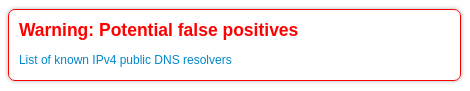
\includegraphics[scale=0.8]{../images/false-positive.png}
\end{frame}

\section{Interesting visual features \\ for analysts}

\begin{frame}
    \frametitle{MISP feature - correlation}
    \begin{itemize}
        \item MISP includes a \textbf{powerful engine for correlation} which allows analysts to discover correlating values between attributes
        \item Getting a direct benefit from shared information by other ISAC members
    \end{itemize}
    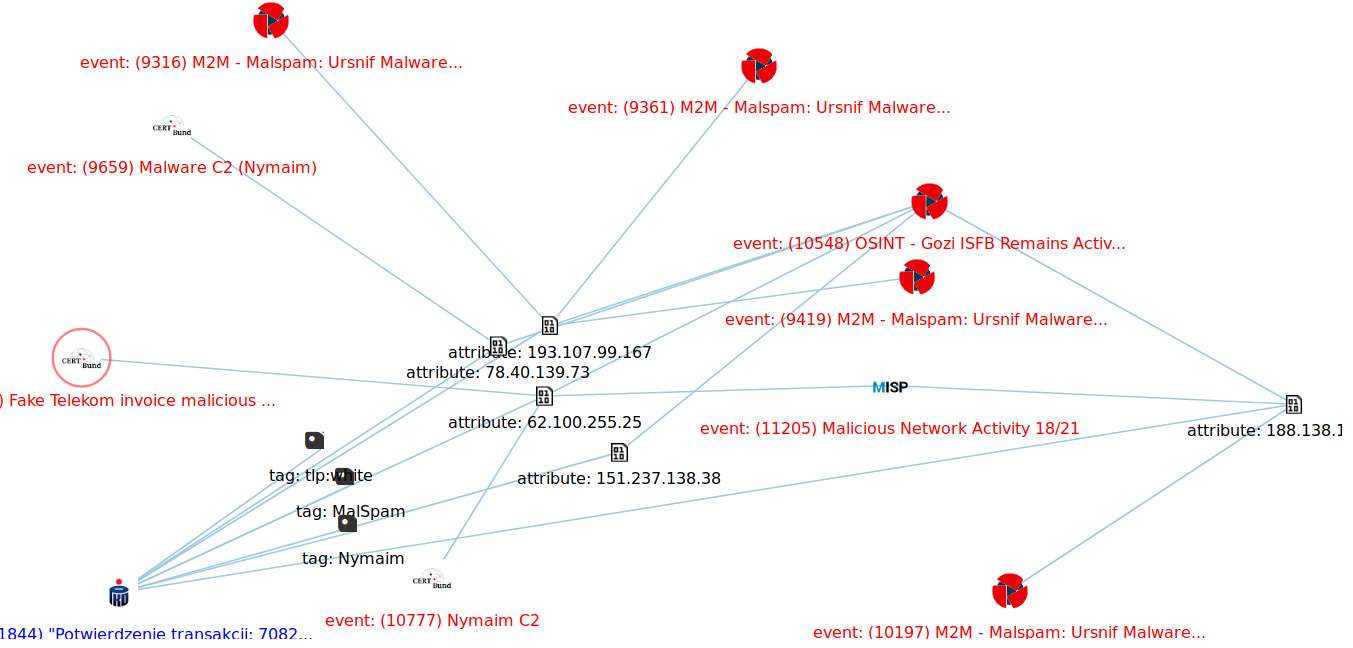
\includegraphics[scale=0.20]{../images/correlation.png}
\end{frame}

\begin{frame}
    \frametitle{MISP feature - event graph}
    \begin{itemize}
        \item \textbf{Analysts can create stories} based on graph relationships between objects, attributes
         \item ISACs users can directly understand the information shared
    \end{itemize}
    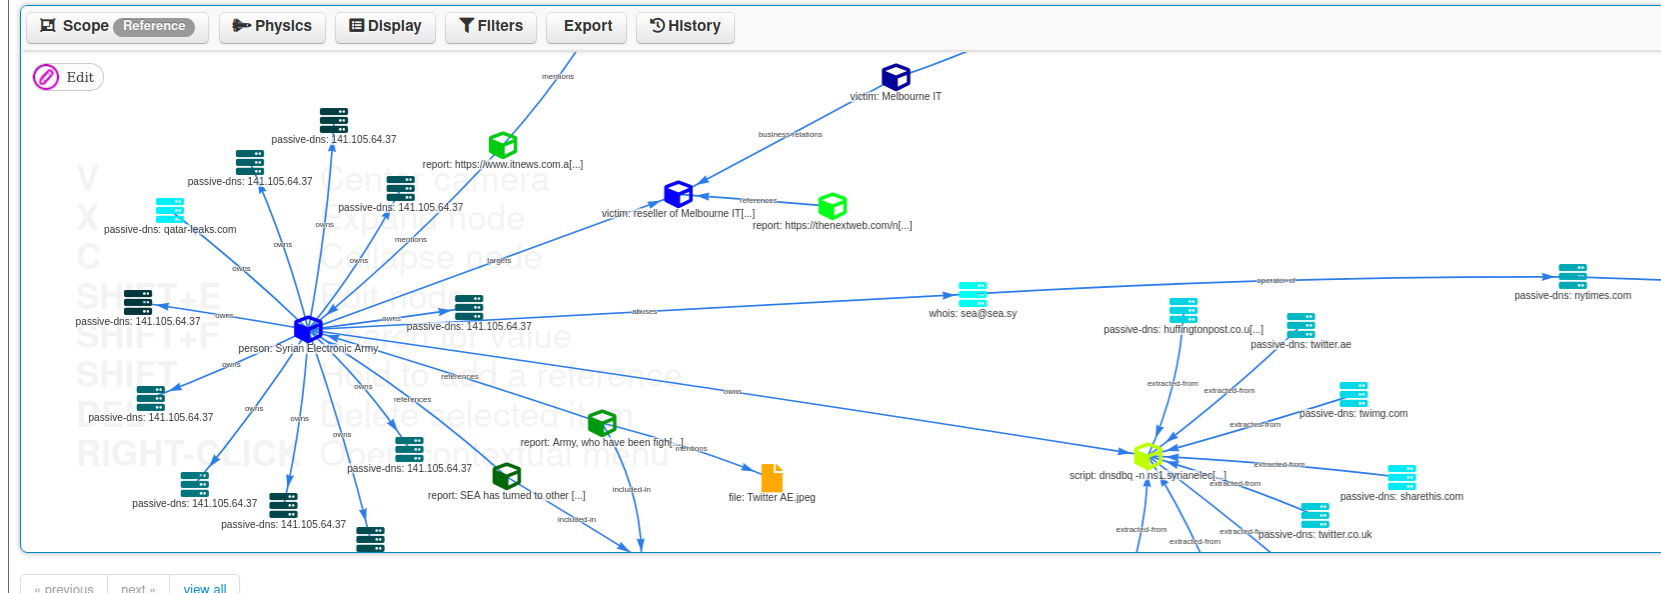
\includegraphics[scale=0.20]{../images/event-graph.png}
\end{frame}

\section{Conclusion}

\begin{frame}
	\frametitle{Conclusion and additional challenges}
	\begin{itemize}
		\item MISP is a complete and advanced tool ...
		\item ... but also \textbf{just one part of the puzzle} in any sharing community
		\item Information sharing presumes knowledge of \textbf{contacts}
		\item Member to Member direct \textbf{exchanges between MISPs and other tools} requires some know how
		\item Creating reusable community-specific \textbf{distribution lists} need to be maintained
		\item Maintaining common \textbf{community specific information knowledgebases} can be challenging
		\item \textbf{Fleet management} for larger organisations needs additional work
	\end{itemize}
\end{frame}

\begin{frame}
	\frametitle{Get in touch if you need some help to get started}
	\begin{itemize}
		\item Getting started with building a new community can be daunting. Feel free to get in touch with us if you have any questions!
		\item Contact: info@circl.lu
		\item \url{https://www.circl.lu/}
		\item \url{https://github.com/MISP}  \url{https://gitter.im/MISP/MISP}  \url{https://twitter.com/MISPProject}
	\end{itemize}
\end{frame}
